% Created 2012-12-17 Mon 03:07
\documentclass[11pt]{article}
\usepackage[utf8]{inputenc}
\usepackage[T1]{fontenc}
\usepackage{fixltx2e}
\usepackage{graphicx}
\usepackage{longtable}
\usepackage{float}
\usepackage{wrapfig}
\usepackage{soul}
\usepackage{textcomp}
\usepackage{marvosym}
\usepackage{wasysym}
\usepackage{latexsym}
\usepackage{amssymb}
\usepackage{hyperref}
\tolerance=1000
\providecommand{\alert}[1]{\textbf{#1}}
\setlength{\parindent}{0cm}

\title{FinalReport}
\author{Bergar Simonsen, Morten Holm Hvass, Filip Hjermind Jensen}
\date{\today}
\hypersetup{
  pdfkeywords={},
  pdfsubject={},
  pdfcreator={Emacs Org-mode version 7.8.11}}

\begin{document}

\maketitle

\setcounter{tocdepth}{3}
\tableofcontents
\vspace*{1cm}
\newpage
\section{Introduction}
\label{sec-0}
This application and report was made at the end of year 2012 at the IT-University of Copenhagen in the context of the final project of the Analysis, Design and Software Architecture course. The project was made under the guidance of our teachers Jakob Eyvind Bardram and Dario Pacino along with our TA's Mads Mærsk Frost and Simon Bang Terkildsen. \\

The solution consists of an application, written in C\# and ASP.NET. Followed by a report, document the application. \\

The report divided into four main parts: \\

The first is the Business Model. The business model gives a short introduction and a quick overview of the system and it's core features. \\
The business model is then followed by the Requirements / Analysis part. This part consists of all the analysis that was in order to make the application. \\
The third part is the Design part. This parts consists of documentation on how we would go about designing our application. \\
The fourth is the implementation part. This part contains specific documentation on our application, along with some design choices made along the way. This part is primarily meant for developers. \\
The final part is the project management part. This part documents how our work process has gone. Document our progress and work flow.

\newpage

\section{Business Modeling}
\label{sec-1}
\subsection{Vision}
\label{sec-1-1}
\subsubsection{Introduction}
\label{sec-1-1-1}

Our goal is to make an interactive document sharing system, Slice of Pie,  which allows multiple users to easily share and edit documents both online and offline
\subsubsection{Problem statement}
\label{sec-1-1-2}

    Sharing and editing documents can be cumbersome. 
    Sending a document back and forth between multiple users can lead to a lot of errors. Users can overwrite what another user has done, and if they aren't all
    using the same text editing system this can lead to formatting issues in the document.
\subsubsection{Summary of system features}
\label{sec-1-1-3}

\begin{itemize}
\item Multiple users must be able to share and edit documents online.
\item Synchronization for offline usage.
\item See \emph{Supplementary Specification} for a more complete list of system features.
\end{itemize}
\subsection{Glossary}
\label{sec-1-2}

\begin{itemize}
\item \textbf{Response Time:} The time it takes for the system to respond to a request from the user.
\item \textbf{Document:} A document refers to a complete document, not just a single file. A document contains a owner, id, content and a file.
\item \textbf{Client:} A client can mean two things. A web client, operating directly on the server, and a stand-alone client, that runs locally on the end users machine synchronizing with the server.
\item \textbf{System:} Refers to the core of the application. This includes document handler, user handler etc ..
\end{itemize}
\section{Requirements / Analysis}
\label{sec-2}
Before starting on the application itself, some analysis had to be made in order to find out how the system will be build. \\
This includes finding out the core functionality of the system as well as finding out some of the non functional requirements for the application. \\
The following is a documentation of the analysis that was made before the development of the application began.
\subsection{Use cases}
\label{sec-2-1}
Use cases show an overview of the features that are available in the system. Below are a list of all use cases that our system supports. \\
\emph{Section 2.1.1} shows a diagram of all fundamental use cases available in the system. \\
See \emph{Appendix} for an elaboration on each use case. \\

\begin{itemize}
\item UC1: Create new document
\item UC2: Edit document
\item UC3: Delete document
\item UC4: Merging documents (resolve conflict)
\item UC5: Offline sync
\item UC6: New folder
\item UC7: New project
\item UC8: Find old version of document
\item UC9: Share Document
\item UC10: Log in
\end{itemize}
\subsubsection{Use case Diagram}
\label{sec-2-1-1}
\begin{figure}[H]
  		\centering
    	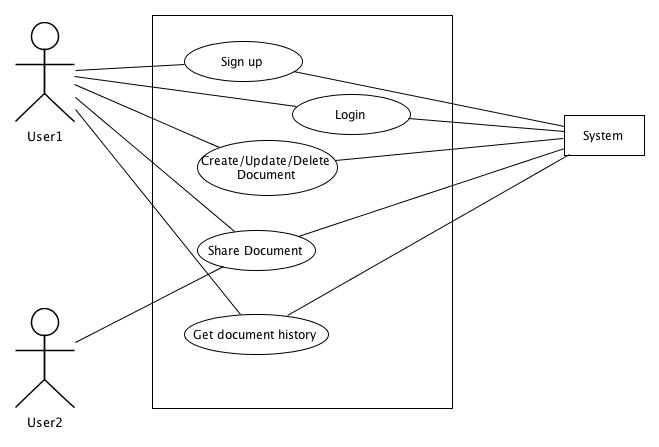
\includegraphics[width=300px]{images/UpdatedUsecaseDiagram.jpg}
    	\caption{Use-case diagram}
	\end{figure}
\subsection{Supplementary Specification (FURPS+)}
\label{sec-2-2}
Supplementary specification, along with use cases, show all the requirements that our system must fulfill.

\begin{itemize}
\item Functionality
\begin{itemize}
\item The system must be able to create/edit/delete users.
\item The system must be able to create/edit/delete/share documents.
\item The system must keep a log of all document actions.
\item All system usage requires user authentication.
\item The system must support multiple users.
\end{itemize}
\item Usability
\begin{itemize}
\item The system must be easy to use.
\begin{itemize}
\item Have a clean user interface.
\item 8 out of 10 users must be able to use the system without any training.
\end{itemize}
\item The system must be easily visible for people with ``not perfect'' vision. 
       E.g no graphics that blurs the view of the core system functionality.
\item The web client must be easy and quick to navigate. No function should 
       be more than 3 clicks (windows/sub-windows) away.
\begin{itemize}
\item Not counting navigating a users files.
\end{itemize}
\end{itemize}
\item Reliability
\begin{itemize}
\item It must be possible to use the system without any internet connection.
\begin{itemize}
\item With some limitations.
\end{itemize}
\end{itemize}
\item Performance
\begin{itemize}
\item The system must respond instantly
\begin{itemize}
\item A request must not take more than a few (2-3) seconds.
\item Not taking external factors (such as bad internet connection) into account.
\end{itemize}
\end{itemize}
\end{itemize}
\newpage
\subsection{Domain Model}
\label{sec-2-3}
The domain model shows the domain that our application operates in. \\
This isn't a complete diagram, but a rough sketch that gives us a platform to work from.
\begin{figure}[H]
  		\centering
    	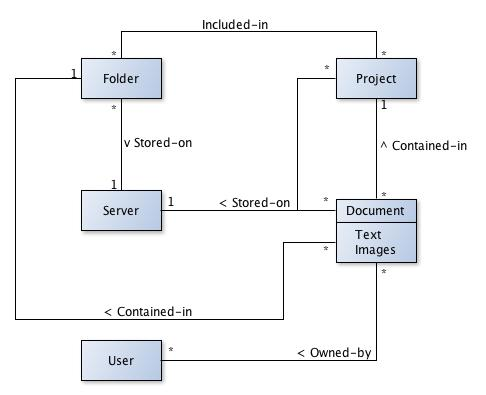
\includegraphics[width=300px]{images/DomainModel.jpg}
    	\caption{Domain Model}
\end{figure}
\newpage
\subsection{Logical Architecture}
\label{sec-2-4}

   The logical architecture diagram shows a rough sketch off how the structure of the application
   will be like. This is by no means a complete diagram, but should give an idea off how
   the application will look like.
\begin{figure}[H]
  		\centering
    	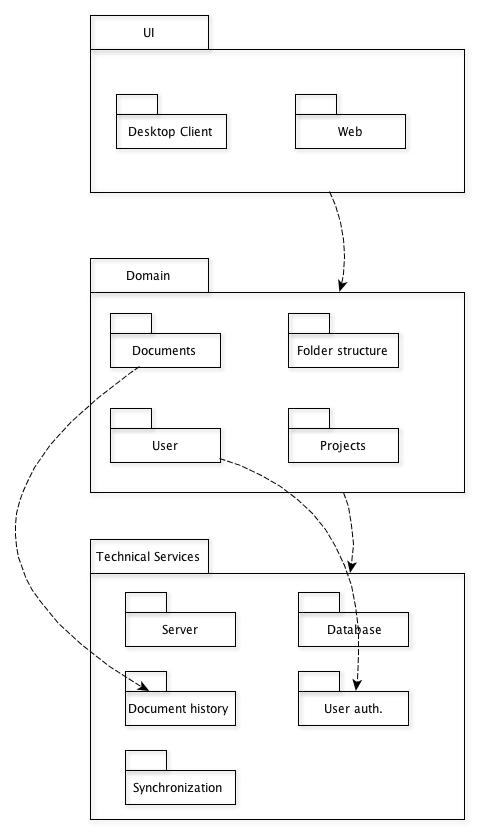
\includegraphics[width=100px]{images/LogicalArchitecture.jpg}
    	\caption{Logical Architecture}
\end{figure}
\subsection{System Sequence Diagram}
\label{sec-2-5}

   The system sequence diagram shows a quick overview of the core functionality available to a end user.
\begin{figure}[H]
  		\centering
    	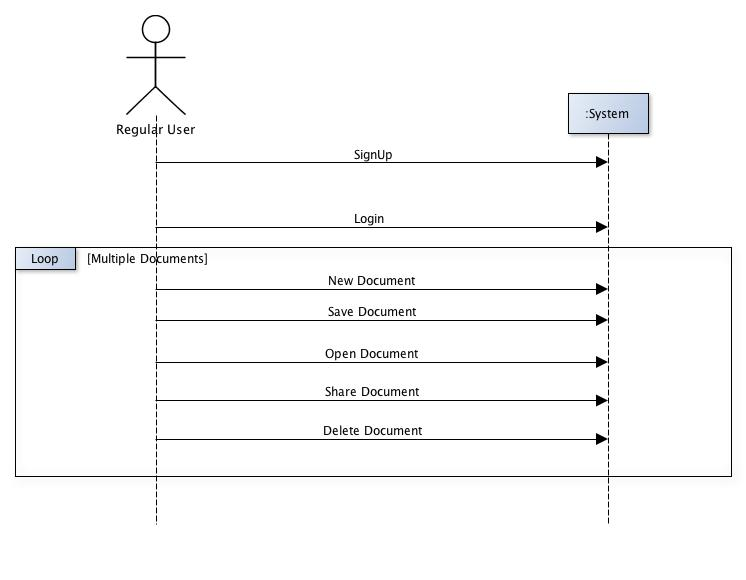
\includegraphics[width=300px]{images/Complete_SSQ.jpg}
    	\caption{System Sequence Diagram}
\end{figure}
\subsection{Operation Contracts}
\label{sec-2-6}
Operation contracts show more details on some of the non trivial use cases of the application. \\
In our application there is only one use case that we thought isn't trivial to the reader. \\
\fbox{\begin{minipage}{\columnwidth}
		\textbf{Contract CO1:} Synchronize / Merge \\
		\textbf{Operation:} Synchronize / Merge \\
		\textbf{Cross References:} UC1, UC2, UC4, UC5 \\
		\textbf{Preconditions:} Some documents and/or folders must have been created on the system. \\
		\textbf{Postconditions:}
		\begin{itemize}
		\item All documents and folders on the client must be uploaded to the server.
		\item All documents and folders on the server must be downloaded to the client.
		\item Document version must be the same on the client and server.
		\end{itemize}
\end{minipage}}

\section{Design}
\label{sec-3}
When the analysis had gotten well underway, we could start to design the application itself. This includes class diagrams, core architecture etc ..
\subsection{Class Diagram}
\label{sec-3-1}
The class diagram show how our server side classes are connected. For a complete class diagram for all classes, along with methods and fields, see the \emph{appendix.}
\begin{figure}[H]
  		\centering
    	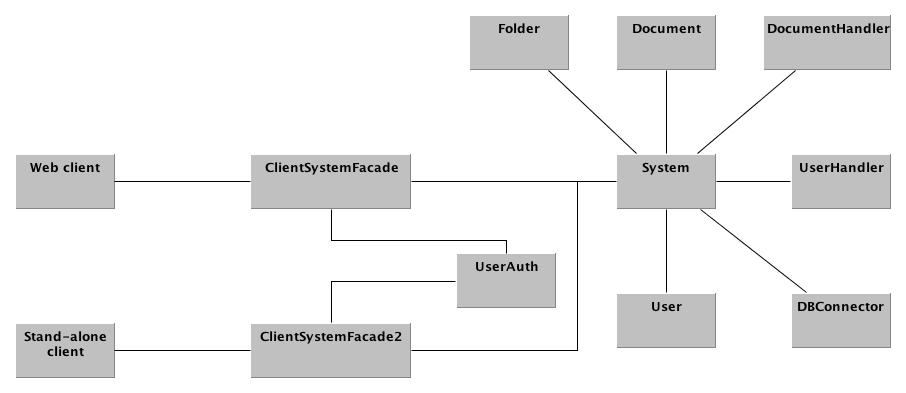
\includegraphics[width=300px]{images/LatestClassDiagram.jpg}
    	\caption{Class Diagram}
\end{figure}
\subsection{Interaction Diagrams}
\label{sec-3-2}
Interaction diagrams show how our application communicates internally in regards to some of our use cases. \\
Not all use cases are covered here, but it should be enough to give an overview of the main features, and elaborate on some use cases that aren't trivial to understand.
\subsubsection{Sequence Diagram}
\label{sec-3-2-1}
The SaveDocument() Sequence Diagram shows how the system communicates internally when the SaveDocument() method is called.
For other related methods (OpenDocument() ShareDocument() etc.. ) the program flow is the same (though they vary on some parameters and other details).
\begin{figure}[H]
  		\centering
    	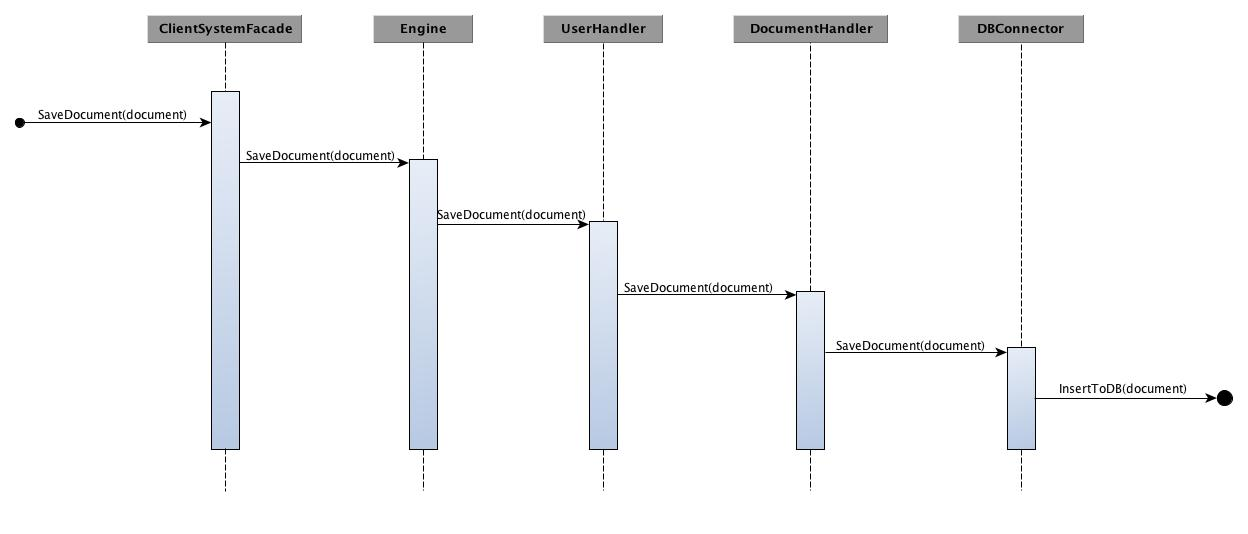
\includegraphics[width=300px]{images/SequenceDiagram_SaveDocument.jpg}
    	\caption{Sequence Diagram}
\end{figure}

\subsubsection{Communication Diagram}
\label{sec-3-2-2}
The communication diagram below shows how our application communicates internally when the synchronize method is called from the stand alone client. 
\begin{figure}[H]
  		\centering
    	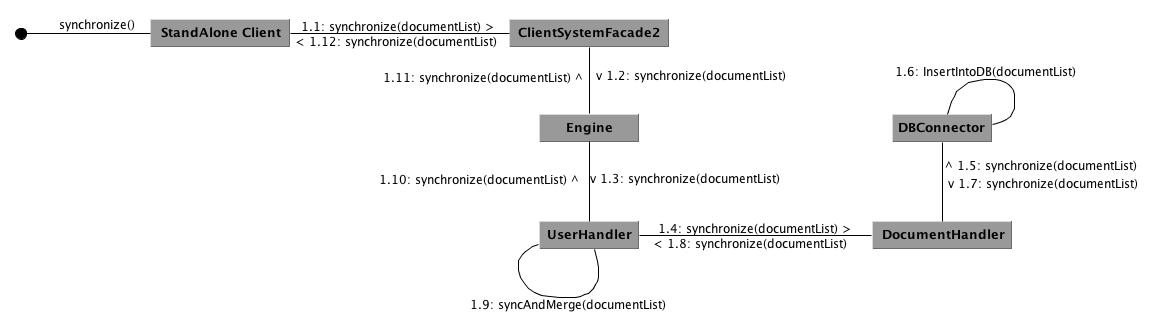
\includegraphics[width=300px]{images/CommunicationDiagram_Synchronize.jpg}
    	\caption{Communication Diagram - Synchronize}
\end{figure}
\newpage
\subsection{ER-Diagram}
\label{sec-3-3}
The ER-Diagram shows the structure of our database design. \\
Note that the \texttt{documenthistory} table isn't used in the final design, but instead we use the \texttt{document} table to store the document history. \\
In a future update the \texttt{documenthistory} table will be implemented.
\begin{figure}[H]
  		\centering
    	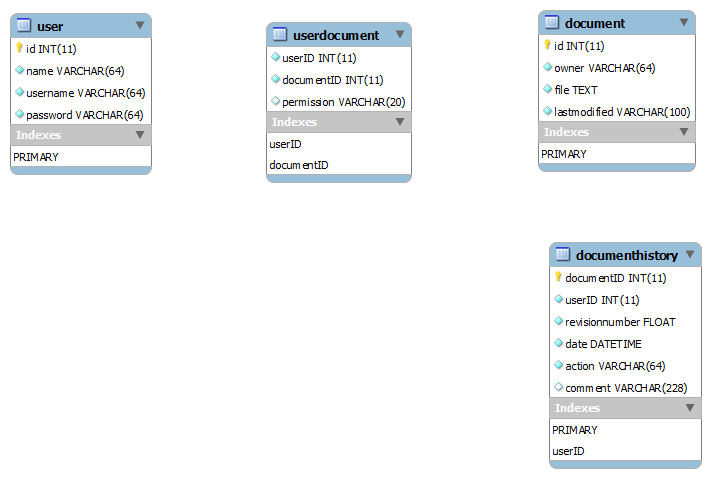
\includegraphics[width=300px]{images/New ER database.png}
    	\caption{ER-Diagram}
\end{figure}
\subsection{User manual}
\label{sec-3-4}
The application should be relatively easy to use but in case there is some confusion on some parts, we wrote a user manual to help the user to get started. \\
This document isn't a complete user guide, but should only be used as a quick start guide to the application. \\
The stand alone client is very trivial, so we neglected writing a manual for it. Therefore the following manual is based on the web client alone.
\subsubsection{Starting the application}
\label{sec-3-4-1}
\begin{itemize}

\item \textbf{Running the application from Visual Studio}\\
\label{sec-3-4-1-1}%
Before starting the application, you need to start Visual Studio with administration privileges.
The reason for this is that the application will need to create files and folders for the documents and in order to do so the program needs to be run with administrator privileges which will give the application write access.

Since the web client runs in the browser, the browser needs to allow pop up windows for localhost.
This can be done when the application is run for the first time.

When starting the application, you need to set the \texttt{WebClient} project as startup project (if it's not already set), and then run the program (f5 for debug mode, ctrl + f5 for the release version).

The web client will start up with your default internet browser. 
When the main page has loaded, you are ready to use the application.

\item \textbf{Signing up} \\
\label{sec-3-4-1-2}%
As a first time user there won't be any user registered in the system, so the first time you need to sign up to use the system.

To sign up, click the \texttt{Sign up} button. This will open up a new window with the sign up form.

Fill out the form and click the \texttt{Sign up} button. A message will appear to say if the sign up was successful or not.

If the sign up was successful you are now registered in the system, and are ready to use it. 
Close the sign up window and go back to the main window.

\item \textbf{Logging in}\\
\label{sec-3-4-1-3}%
On the main screen there are two text boxes at the top of the window named "username'' and "password''.
Enter the newly created username and password into the boxes and click the \texttt{Login} button.
\end{itemize} % ends low level
\subsubsection{Using the Application}
\label{sec-3-4-2}

After you have logged in, press the \texttt{Get Files} button on the left page of the window. 
This will show you all the files that belong to the current user. Since you are a new user you don't have any documents, so you should only see the root folder (the one with your username).
\begin{itemize}

\item \textbf{Create a new document}\\
\label{sec-3-4-2-1}%
To create a new document, click the \texttt{New Document} button. This will clear all text boxes, and you are ready to write a new document.

Creating a new document doesn't save the document, so before you go too far you should save your document.
Write a file name in the file name box, and click the \texttt{Save Document} button.
If you wish to save the document in a sub folder, just write: "folder name/file name.html'' in the file box.

The system doesn't require that you save the document as a HTML file, but the system is built around it. Not doing so won't make it able to add images to you document.

\item \textbf{Deleting a document} \\
\label{sec-3-4-2-2}%
Deleting a document is very simple.
Select a document from the list on the left. Make sure that the filename of the file is entered into the file name box (this can also be done manually). Delete the document by clicking the \texttt{Delete Document} button.

\item \textbf{Sharing a document} \\
\label{sec-3-4-2-3}%
Sharing a document is very simple as well. \\
Open the document you wish to share. Enter the user name of the user you wish to share the document with in the text box next to the \texttt{Share Document} button, and click the \texttt{Share Document} button.

\item \textbf{Showing a document} \\
\label{sec-3-4-2-4}%
Since the document is built around the HTML format, the text area can't show any images or text formatting.
In order to see the document (with images, formatting etc) you need to open it in another page in the browser.
Select the document you wish to view and click the \texttt{Show Document} button. This will open a new window with your document in parsed HTML.

\item \textbf{Showing a document's history} \\
\label{sec-3-4-2-5}%
When multiple users work on the same document it can be very useful to see a change log of the document. \\
To see a log of all changes made to a document, select a document from the file list and click the \texttt{Show Document History} button. This will open up a new window which shows a log of when the system has been changed.
\newpage
\end{itemize} % ends low level
\section{Implementation}
\label{sec-4}
The implementation part documents how we have implemented our application. \\
The following sections show various diagrams and design choices we have made during the development of the application. \\
These artifacts can be found in the Software Architecture Document.
\subsection{Software Architecture Document}
\label{sec-4-1}
The Software Architecture Document (SAD) is meant for developers that want to learn about the different implementation of our system, or maybe want to extend our system. \\
If you wish to read about the different design choices etc then please read on, otherwise you might want to skip this part.
\subsubsection{Architectural Representation}
\label{sec-4-1-1}

The SAD summarizes the architecture of the Slice of Pie application from multiple views. These views include:
\begin{itemize}
\item Logical view
\item Deployment view
\item Process view
\item Data view
\item Use-case view
\end{itemize}
\subsubsection{Architectural Factors}
\label{sec-4-1-2}
\emph{See section 2.2 - Supplementary requirements}
\subsubsection{Architectural Decisions}
\label{sec-4-1-3}
Architectural decisions describe some of the decisions that we took in our design. Our decisions (and motivation for the decisions) are shown as technical memos.

\label{sec-4-1-3-1}%
\fbox{\begin{minipage}{\columnwidth}
\begin{center}
\textbf{Technical Memo} \\
\end{center}
\textbf{Issue:} Files format - Which file format to use \\
\textbf{Solution Summary:} Use HTML for our file format. \\
\textbf{Factors:}
\begin{itemize}
\item Must be able to contain both text and images.
\end{itemize}
\textbf{Solution:}
We chose to use HTML for our file format because it's simple to construct, and can contain text and images seamlessly. \\
\textbf{Motivation:} \\
We needed a file format that can contain images and text as well as being easy to construct. in addition, HTML can easily be extended to other content. \\
Lastly, HTML can be opened with any browser, so the users isn't tied to SliceOfPie if he just want's to view the content of a file. \\
\textbf{Alternatives considered:} \\
We considered using a .txt file format, but .txt can only contain plain text.
We also considered using our own file format (since the format itself isn't important to the application). But if we use our own format the user is stuck
with using SliceOfPie, so he can't view the content of a file with any other application.
\end{minipage}}

\fbox{\begin{minipage}{\columnwidth}
\begin{center}
\textbf{Technical Memo} \\
\end{center}
\textbf{Issue:} Merging two versions of the same document. \\
\textbf{Solution Summary:} Git-hub inspired merge. \\
\textbf{Factors:}
\begin{itemize}
\item Merging two versions of the same document without overwriting existing changes.
\end{itemize}
\textbf{Solution:}
Our merging algorithm reads the two documents and stores them, line by line in an array.  \\
Then the algorithm compares each line in the two arrays, if the lines are the same, insert the line into a new array. If the two lines aren't identical, insert the new line into the new array + insert the line from the old array in the next line. This line will be encapsulated with $<<<$ TEXT $>>>$ which shows the user where there is a conflict which the user can solve later on. 
If the new version of the document contains lines that aren't in the old array, they are simply added to the new array. \\
\textbf{Motivation:} \\
There are other, more advanced, merging algorithms available. Because of time constraint we chose to use this one. It isn't the most advanced/complete algorithm but it does the job quite well considered it's simplicity. \\
\textbf{Unresolved issues:} 
\begin{itemize}
\item Our algorithm doesn't 100\% solve the conflict. In the end the user must manually chose which version to keep, and which version to discard.
\item If two identical lines exists in both versions but the lines is at another line number in the old document, this might cause a conflict $<<<$ TEXT $>>$ that could be avoided.
\end{itemize}
\textbf{Alternatives considered:} \\
An algorithm that analyses every line in the file keeps the one that the user wants.
\end{minipage}}

\fbox{\begin{minipage}{\columnwidth}
\begin{center}
\textbf{Technical Memo} \\
\end{center}
\textbf{Issue:} Choosing how to connect to the database \\
\textbf{Solution Summary:} Simplest option due to time pressure \\
\textbf{Factors:}
\begin{itemize}
\item Simplicity
\item Easy to get working
\end{itemize}
\textbf{Solution:} \\
Our way of connecting to the database, and executing queries on it is a series of methods close to hard coded SQL queries. They do not automatically update if a table/column/attribute were to change. \\
\textbf{Motivation:} \\
Early in the process we also designed a solid design for the database, which meant that we were able to make the "final'' outcast of the database rather quickly. \\
And looking apart from the fact that the solution does not adapt to changes made on the database, it works perfectly and required minimal attention and time to get working. \\
\textbf{Alternatives considered:} \\
Entity framework was a possibility from the start, but since entity framework had proven a challenge to get working for all of us in the past, we choose the, for us at the time, simpler solution to save time in the end
\end{minipage}}



\subsubsection{Logical View}
\label{sec-4-1-4}
The logical view shows the architectural structure of our application. \\
Note that the "packages" not necessarily are programming packages/projects but should be thought of as subsystems or modules.

\begin{figure}[H]
  		\centering
    	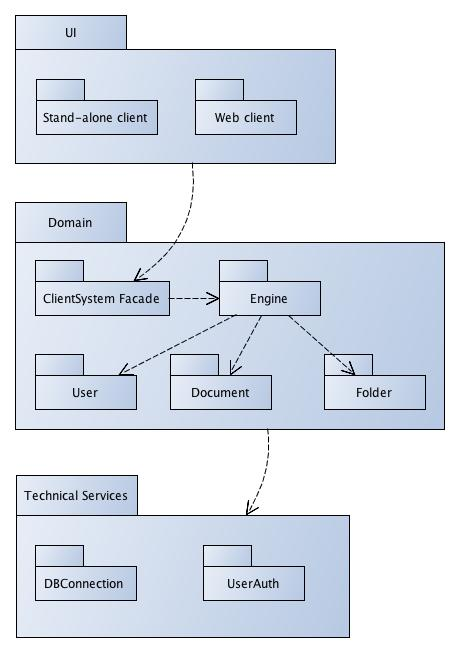
\includegraphics[width=300px]{images/SAD/LogicalView_UML.jpg}
    	\caption{Logical View}
\end{figure}

\subsubsection{Deployment View}
\label{sec-4-1-5}
The deployment view shows how our application is deployed when it's released. The actual application hasn't been released so this is to be thought of as the most likely structure when it is released.

\begin{figure}[H]
  		\centering
    	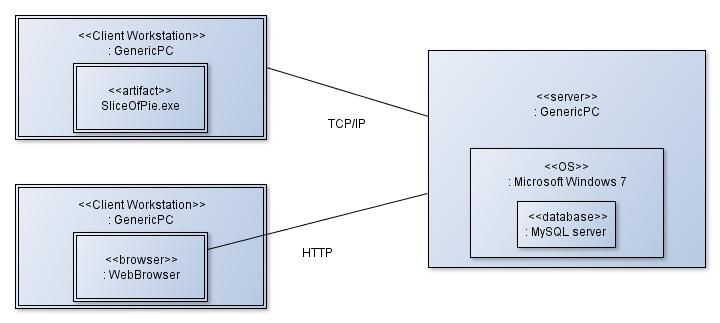
\includegraphics[width=300px]{images/Deployment Diagram.jpg}
    	\caption{Deployment Diagram}
\end{figure}
\subsubsection{Process View}
\label{sec-4-1-6}
Process view shows how our application communicates internally. It shows how the classes operate with each other when performing various functions. \\
Note that not all process diagrams are shown here, see \emph{Section X - Communication Diagrams} for more diagrams

\begin{figure}[H]
  		\centering
    	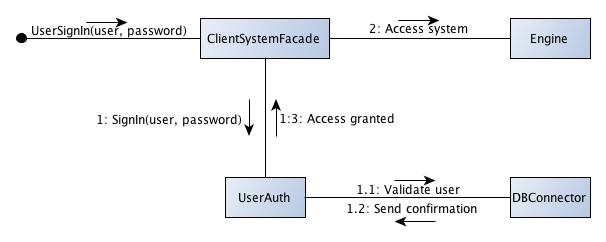
\includegraphics[width=300px]{images/SAD/CommunicationDiagram_LogIn.jpg}
    	\caption{Communication Diagram - Log in}
\end{figure}

\begin{figure}[H]
  		\centering
    	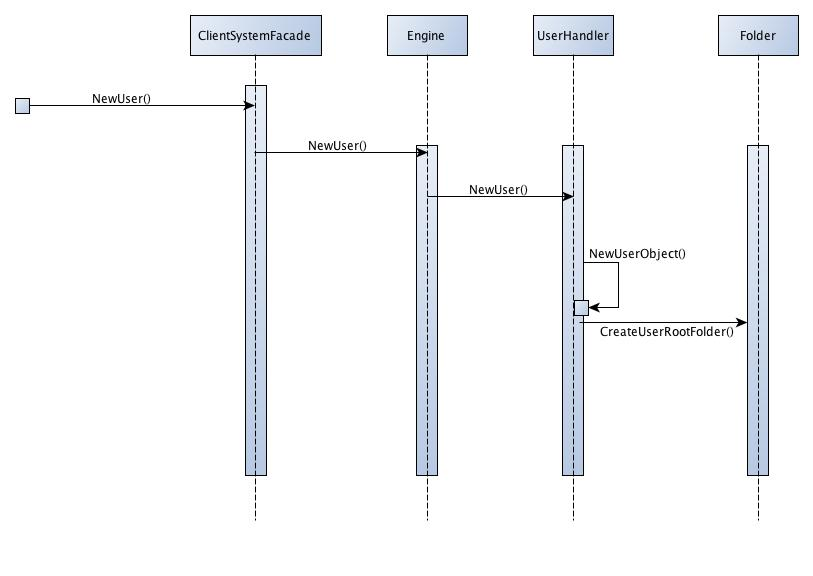
\includegraphics[width=300px]{images/SAD/SSQ_NewUser.jpg}
    	\caption{Sequence Diagram - New User}
\end{figure}

\begin{figure}[H]
  		\centering
    	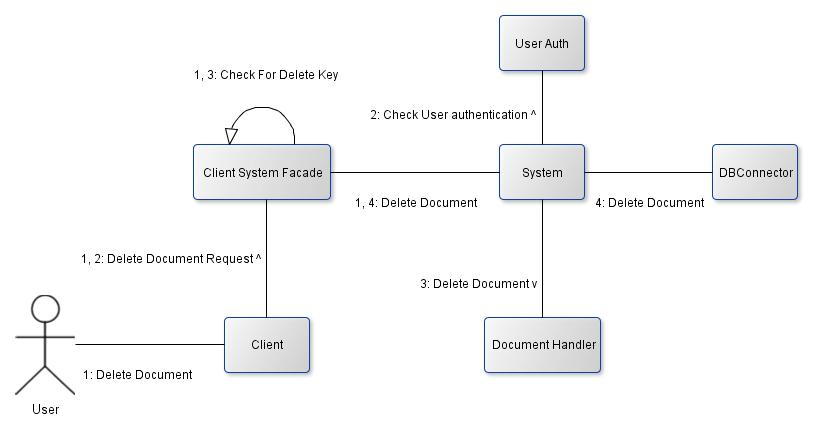
\includegraphics[width=300px]{images/CommunicationDiagrams/Delete Communication Diagram.jpg}
    	\caption{Communication Diagram - Delete Document}
\end{figure}

\subsubsection{Use-Case View}
\label{sec-4-1-7}

See \emph{Section X - Use cases}

\subsubsection{Known Issues}
\label{sec-4-1-8}
While our system isn't a finished product but a proof of concept or prototype of the finished product, there are some known issues or bugs that can occur in the application. \\
Below is a list of some of the known issues currently in the application. \\ ~\\
\textbf{Web Client} 
\begin{itemize}
\item The File Tree doesn't update after a change has been made. The user has to click the 
     Get Files button every time a document is created or deleted.
\item Since the File Tree doesn't update itself it won't remove it self either. Clicking
     the Get Files button won't remove the existing File Tree but makes a new one. 
     The old one can then be ignored.
\item Saving a shared document isn't 100\% optimal. 
     When saving a shared document, it creates a new document in the current users 
     name. To allow the ``other'' user of the document to get the changes made to
     the shared document, you need to share it again, with the changes.
\item Every time a document is saved, and extra line break is added to each line. Since
     the document is based on HTML this has no effect on the outcome of the final 
     document, but can be annoying to look at.
\item Getting files sometimes takes longer than we anticipated.
\begin{itemize}
\item The reason for this is because of the shared documents. We waited until the end 
       to implement the shared documents. Because of this we had to make some ``hacks''
       in order to get it done by the deadline.
       If we had more time this would be implemented otherwise.
\end{itemize}
\end{itemize}
\textbf{Stand-Alone Client} 
\begin{itemize}
\item Creating files in the ``root-root'' folder if no folder is selected, the 
     ``create document'' method creates a document in a folder that should not 
     be accessible at all
\item ``Update settings'' creates new directory, even if user does not exist.
     When calling the method, it takes the ``username'' and creates a new folder 
     in currently selected directory
\item No way to log in on the standalone client, if your credentials are in the 
     ``username'' and ``password'' textboxes, this is considered logging in.
\item When synchronizing, the document will not be successfully synchronized the first time
     and the user will not be told when is is done, only the server can see if the
     documents have been successfully synchronized.
\item When synchronizing files that do not yet exist on the server, the server needs time 
     to create the files, this blocks the client from receiving the files, this results in
     the client only getting existing documents on server back.
\item Synchronize() should return a boolean, describing whether the sync was successful or not
     most times when not successful it is because of the above problem
\item It is possible to synchronize but it often takes more than one attempt. You will get some errors in the console, they can safely be ignored. Just try again.
\end{itemize}
\newpage
\section{Project Management}
\label{sec-5}
\subsection{SCRUM}
\label{sec-5-1}
For managing our work process, we have been using the SCRUM developing method. \\
The next sections describe some documentation and artifacts that document how our process has developed when working on the project. \\
Note that not all artifacts are shown here, some references are to the appendixes. \\

Before our system is ready for release, we must have implemented all required features. \\
In addition to implementing the features, we also must document every aspect of the system and the process. This includes diagrams, use cases etc \ldots{} \\
Finally we have to test our system to make sure that it works as intended and doesn't break when run. \\

\subsubsection{Definition of done}
\label{sec-5-1-1}

To keep track of how the system is coming along, and to decide when the application can be deemed done, we have written a definition of done. \\
The definition of done acts as a checklist that shows how far along in the process we are, and how far we have yet to go. \\

\textbf{Development} \\
\label{sec-5-1-1-1}%
The system must be able to handle all the requirements before it can be deemed done. \\
These requirements include the assignment required requirements as well as our own requirements. \\

These requirements include:
\begin{itemize}
\item $\boxminus$ Document [3/4]
\begin{itemize}
\item $\boxtimes$ Create a document that can handle both text and images.
\item $\boxtimes$ Documents can be arranged into folders.
\item $\Box$ Documents can be arranged into projects (optional). (skipped)
\item $\boxtimes$ Log of all changes to a document.
\end{itemize}
\item $\boxtimes$ System [4/4]
\begin{itemize}
\item $\boxtimes$ Synchronization for offline usage.
\item $\boxtimes$ Sharing of documents to other users.
\item $\boxtimes$ Authentication system for users.
\item $\boxtimes$ Document storage in a database.
\end{itemize}
\item $\boxtimes$ User Interface [2/2]
\begin{itemize}
\item $\boxtimes$ Web interface.
\item $\boxtimes$ Stand-alone client (for offline usage).
\end{itemize}
\end{itemize}

\textbf{Documentation} \\
\label{sec-5-1-1-2}%
All aspects of the system must be documented. \\
The idea of the documentation is that the system is easy to understand based only on the documentation. \\
In addition, an external actor must be able to see the development
process from reading the documentation only. \\

These documents must be made before the documentation can be deemed as done:
\begin{itemize}
\item $\boxtimes$ Use cases [3/3]
\begin{itemize}
\item $\boxtimes$ All use cases must be documented (text form)
\item $\boxtimes$ Use case diagram must be made for use cases that require it.
\item $\boxtimes$ Operation contracts must be made for use cases that are complex.
\end{itemize}
\item $\boxtimes$ Domain documentation [2/2]
\begin{itemize}
\item $\boxtimes$ A model must be made for describing the domain.
\item $\boxtimes$ A sequence diagram must be made for understanding how the domain interacts.
\end{itemize}
\item $\boxtimes$ Software documentation [4/4]
\begin{itemize}
\item $\boxtimes$ Static class diagram that explains the entire system.
\item $\boxtimes$ Package diagram that shows a higher view of the system.
\item $\boxtimes$ Interaction diagrams that describe the dynamic aspect of the system.
\item $\boxtimes$ E-R diagram for the database structure.
\end{itemize}
\end{itemize}

\textbf{Testing} \\
\label{sec-5-1-1-3}%
Before the system can be declared done, all the core features of the system
must be thoroughly tested.\\
This includes testing all core features of the system. \\

Testing checklist:
\begin{itemize}
\item $\boxtimes$ System [7/7]
\begin{itemize}
\item $\boxtimes$ Document
\item $\boxtimes$ DocumentHandler
\item $\boxtimes$ Folder
\item $\boxtimes$ User
\item $\boxtimes$ UserAuth
\item $\boxtimes$ DBConnector
\item $\boxtimes$ ClientSystemFacade
\end{itemize}
\end{itemize}

\subsubsection{Product Backlog}
\label{sec-5-1-2}
In order to save space, we have put our product back log in the appendixes. Please see appendix X to see the product backlog.
\subsubsection{Sprint Intro}
\label{sec-5-1-3}
We divided the working process itself up into SCRUM sprints. \\
Each sprint lasts for one week. At the end of  each sprint, the idea is to have a system, limited as it may be, that is ready to be released. \\
In total we had 3 sprints + plus a smaller sprint at the end where we connected the remaining parts of the application and finished up some rough edges. \\
Below is a documentation of our three sprints, along with burn down charts, that show how well the process is coming along in relation to the planned schedule.
\subsubsection{Sprints}
\label{sec-5-1-4}

\textbf{- 1. sprint} \\
%\label{sec-5-1-4-1}%
\textbf{Sprint Backlog:} Please see \emph{Appendix X for the sprint backlog.}

\begin{figure}[H]
  		\centering
    	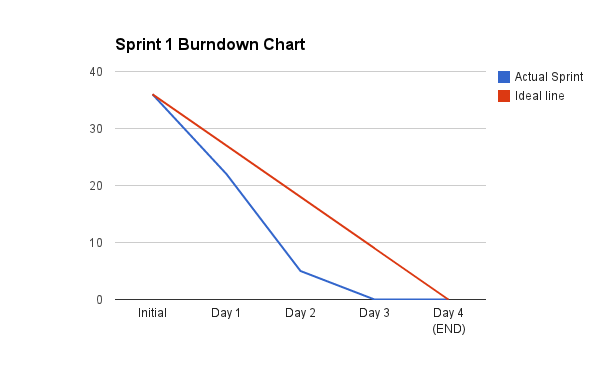
\includegraphics[width=300px]{images/SCRUM/Sprint 1 burndown chart.png}
    	\caption{Sprint 1 burn down chart}
\end{figure}

\textbf{Review:}
\begin{itemize}
\item Items were completed easier than first anticipated
\item To few items in sprint
\item Basic understanding of systems functionality is now documented in form of use cases
\end{itemize}
\textbf{Retrospective:}
\begin{itemize}
\item Group works together great
\item Private lives (jobs, other classes, sports, etc.) interfering with most available
         ``Work-days'', group members are trying to postpone future non-project related activities
\end{itemize}

\textbf{- 2. sprint} \\
%\label{sec-5-1-4-2}%

\textbf{Sprint Backlog:} Please see \emph{Appendix X for the sprint backlog.}

\begin{figure}[H]
  		\centering
    	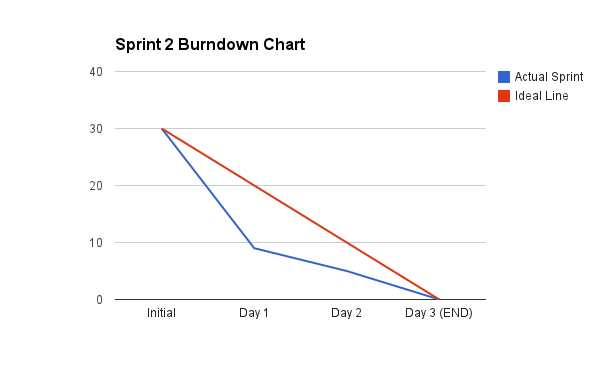
\includegraphics[width=300px]{images/SCRUM/Sprint 2 burndown chart.png}
    	\caption{Sprint 2 burn down chart}
\end{figure}

     \textbf{Review:}
\begin{itemize}
\item Items were easier completed than first anticipated
\item To few items in sprint
\item Started coding for real
\item Basic system architecture taking form
\end{itemize}
     \textbf{Retrospective:}
\begin{itemize}
\item Members finishing their private arrangements (jobs, other classes, sports, etc.)
       Getting more time from next sprint on
\end{itemize}

\textbf{- 3. sprint} \\
%\label{sec-5-1-4-3}%

\textbf{Sprint Backlog:} Please see \emph{Appendix X for the sprint backlog.}
\begin{figure}[H]
  		\centering
    	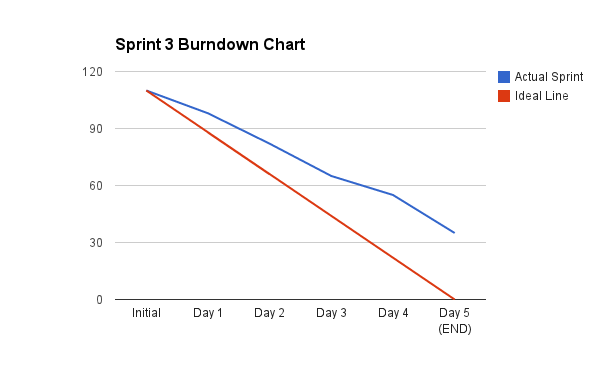
\includegraphics[width=300px]{images/SCRUM/Sprint 3 burndown chart.png}
    	\caption{Sprint 3 burn down chart}
\end{figure}

     \textbf{Review:}
\begin{itemize}
\item Items took longer than expected to complete
\item Finished building separate code, started to implement main features using each other
       instead of test data, encountered more errors than expected and will take al ot of
       work to fix
\end{itemize}

     \textbf{Retrospective:}
\begin{itemize}
\item Members had most time free to work on project, but due to unexpected errors
       sprint was not successfully finished
\item Members still working great together, despite the pressure
\end{itemize}


\textbf{- Final Sprint} \\
%\label{sec-5-1-4-4}%
\textbf{Review:}
\begin{itemize}
\item Most optional functionality were not implemented due to the lack of time
\item All required functionality completed, though with small ``bugs/features''
\end{itemize}

     \textbf{Retrospective:}
\begin{itemize}
\item Members used all spare time they had on the project, but had to drop
       a lot of ``optional work'' to get the program done.
\item Writing the report happened too late according to plan (due to the program
       not being done), but scrum has been followed up on every ``work-day''
       which made the report-writing quite easier.
\end{itemize}
Figure 17 below shows the final release burn chart. \\
As you can see, the ends don't quite meet each other but they were connected the days following the final sprint.
\begin{figure}[H]
  		\centering
    	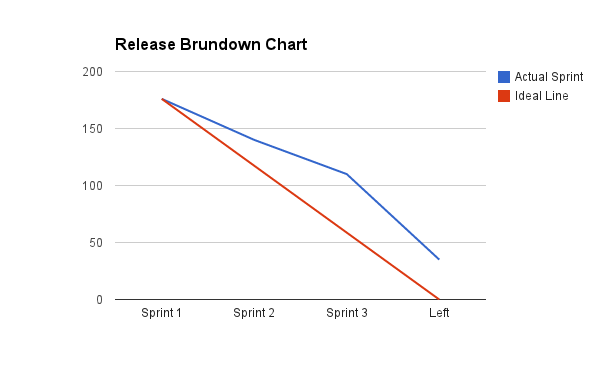
\includegraphics[width=300px]{images/SCRUM/release burn.png}
    	\caption{Sprint 2 burn down chart}
\end{figure}

\subsubsection{Review}
\label{sec-5-1-5}

    The last sprint was chaotic for the members, since their last normal sprint 
    took longer than expected, due to this no sprint backlog was created since 
    most work was getting individually coded function to cooperate.
    Had it not been for a slow start the team would have had a more descriptive
    finishing sprint, and a more linear release burn down chart.
    
    Most of this is caused by the number of members in the team/group, and their 
    experience in being a ``SCRUM-Master'', since there were only 3 members, 
    there was not capacity for only one of the members to be SCRUM-Master.
    
    And without one single SCRUM-Master it was hard for the group to calculate
    the effort of each backlog item. Most of the Team's problems could have been
    solved by better planning more in the beginning of the project, and more time set 
    aside for the actual planning of each sprint.
    
    Private lives also interfered in the project, and this could be avoided by each
    member planning more carefully what they need to do in the project time period 
    

\end{document}
